\documentclass[11pt,a4paper]{article}
\usepackage[T1]{fontenc}
\usepackage[margin=1in]{geometry}
\usepackage{microtype}
\usepackage{amsmath,amssymb}
\usepackage{setspace}
\usepackage{newtxtext,newtxmath}
\usepackage{booktabs}
\usepackage{longtable}
\usepackage{graphicx}
\usepackage{float}
\usepackage{afterpage}
\usepackage{hyperref}
\usepackage{siunitx}
\usepackage{caption}
\usepackage{subcaption}
\usepackage{tabularx}
\usepackage{enumitem}
\usepackage{xcolor}
\usepackage[section]{placeins}
\usepackage[numbers,sort&compress]{natbib}
\captionsetup{font=small,labelfont=bf,skip=5pt,justification=justified,singlelinecheck=false}
\makeatletter
\def\fps@figure{!htbp}
\def\fps@table{!htbp}
\makeatother

% ── Custom math commands ──
\newcommand{\Composite}{\text{Composite}}
\newcommand{\Index}{\text{Index}}
\newcommand{\Volatility}{\text{Volatility}}
\newcommand{\AccScore}{\text{AccScore}}
\newcommand{\Stall}{\text{Stall}}

\title{Fragile Booms in Cities\\[4pt]
\large Temporal Asymmetry in Urban Adjustment}
\author{MACRO-City Engine Research Team}
\date{March 26, 2026}

\begin{document}
\maketitle

% ── Global layout parameters ──
\setstretch{1.16}
\raggedbottom
\setcounter{topnumber}{4}
\setcounter{bottomnumber}{3}
\setcounter{totalnumber}{6}
\renewcommand{\topfraction}{0.9}
\renewcommand{\bottomfraction}{0.85}
\renewcommand{\textfraction}{0.06}
\renewcommand{\floatpagefraction}{0.72}
\setlength{\textfloatsep}{10pt plus 2pt minus 2pt}
\setlength{\floatsep}{8pt plus 2pt minus 2pt}
\setlength{\intextsep}{8pt plus 2pt minus 2pt}

% ── Prevent large blank pages before floats ──
\renewcommand{\dblfloatpagefraction}{0.7}
\setlength{\dbltextfloatsep}{8pt plus 2pt minus 2pt}

\begin{abstract}
Rapid urban growth is often read as evidence of durable development, yet cities can expand visibly while simultaneously accumulating downside risk.
We define this configuration as a \emph{fragile boom}: an urban state in which growth systematically outpaces structural adjustment, so that the fast margins of expansion move before slower urban fundamentals catch up.
Using a harmonized panel of 295 cities across 136 countries from 2015 to 2025, we show that urban adjustment is temporally asymmetric: fast activity signals respond on impact, while slower proxies of structural change adjust with delay and in policy-specific ways.
These temporal gaps matter empirically. In held-out state-classification tests the fragile-boom state improves discrimination relative to static baselines, and in the standardized OECD subset with observed metropolitan PPP GDP it carries forward-looking information about subsequent slowdown, although the external bridge remains bounded rather than universal.
Policy evidence is correspondingly interpreted through timing structure rather than through a single pooled effect: audited policy timing, design-sensitive pooled estimators, and policy-type contrasts are most informative about dynamic response geometry.
The paper therefore argues that visible growth can systematically overstate short-run success when expansion outruns adjustment, and that urban policy is most informative when read through temporal asymmetry rather than through one average coefficient.
\end{abstract}
\noindent\textbf{Keywords:} fragile boom; temporal asymmetry; urban adjustment; city-level monitoring; policy timing; external validation

%==============================================================================
\section{Introduction}
%==============================================================================

\subsection{Motivation}
More than half the world's population now lives in cities, and urban areas generate over 80\% of global GDP \citep{glaeser2011triumph,duranton2015growing}.
Yet urban growth is rarely monotonic: accelerations and slowdowns are episodic, often nonlinear, and difficult to predict \citep{hausmann2005growth,eichengreen2012slowdown}.
The ``middle-income trap'' literature documents the same pattern at the national scale---rapid growth phases can end abruptly, and apparently successful trajectories can stall \citep{hidalgo2007product}.
At the city level, the puzzle takes a distinctive form: some places continue to look prosperous even as transition risk builds underneath.
Cities do not become fragile only when growth stops; they become fragile when structural adjustment lags behind growth itself.

We term this configuration a \emph{fragile boom}: an urban state in which expansion systematically outpaces adjustment, so that cumulative downside risk builds while visible growth continues.
The empirical intuition is a temporal separation between faster and slower urban signals.
Fast indicators---activity intensity, emissions, operational mobility---can move quickly around shocks, whereas slower signals linked to built form and physical urban expansion adjust with delay (Fig.~\ref{fig:event_study_dynamic}).
Conventional empirical designs tend to blur this timing because they summarize heterogeneous margins of adjustment as if they moved on comparable timescales.

To examine that problem, we assemble a global panel of 295 cities and use it to trace how risk states, policy timing, and spatial exposure evolve over time.
The central question is narrower than a universal policy-effect claim: when visible urban growth and underlying adjustment diverge, which monitored signals reveal the mismatch, and how far can currently auditable policy evidence go in explaining the timing of that divergence?

\subsection{Contributions}
This paper makes four linked contributions.
First, it defines \emph{fragile boom} as a measurable urban risk state rather than a loose descriptive metaphor.
Second, it documents a temporally asymmetric pattern of urban adjustment in which fast signals move first and slower adjustment proxies follow later.
Third, it shows that policy responses differ systematically by type, so infrastructure, digital, and environmental interventions leave distinct timing profiles that are obscured by pooled averages alone.
Fourth, it provides a bounded external bridge by linking fragile-boom states to observed metropolitan GDP slowdown in a standardized OECD subset while keeping broader country-year endpoints clearly separated from city-level validation.

The paper proceeds in a simple sequence: we first establish the measurement setting and transition-risk states, then validate those states against observed GDP, next examine policy-timing diagnostics under audited treatment assignment, and finally test how far the main descriptive patterns survive spatial and design-based stress tests.

\begin{figure}[H]
  \centering
  \fbox{%
    \parbox[c][0.26\textheight][c]{0.94\textwidth}{%
      \centering
      \textbf{Figure Placeholder}\\[4pt]
      Conceptual flowchart temporarily removed for redesign.\\
      Final version should summarize the empirical logic from multi-modal urban observation to\\
      fast/slow signals, fragile-boom diagnosis, bounded external validation, and policy timing.
    }%
  }
  \caption{Empirical logic of the paper. The analysis moves from multimodal city observation to temporally differentiated fast and slow signals, fragile-boom diagnosis, bounded external validation, and policy/spatial diagnostics.}
  \label{fig:evidence_chain}
\end{figure}
\FloatBarrier

Figure~\ref{fig:evidence_chain} summarizes this logic before the paper turns to the data, the external bridge, and the main timing results.

\subsection{Interpretive scope}
Because the paper combines state measurement, external validation, event-study evidence, and spatial diagnostics, interpretation is organized by evidence tier rather than forced into one claim.
Predictive performance is therefore read as evidence about forward-looking state information rather than causality.
The policy layer is constrained further by treatment assignment: audited direct-core events are anchored to registry-dated policy onset, and many correspond to regionally concentrated urban programs whose implementation is shared across the cities most exposed to them.
The present design is therefore strongest for shared timing diagnostics and weaker for within-country rollout intensity.
Policy-type event studies on observed outcomes are read accordingly: they are most informative about timing geometry and cross-bucket differences, while pooled scalar estimates are treated as secondary summaries rather than definitive policy parameters \citep{athey2019machine,mullainathan2017machine,imbenwooldridge2009recent}.
When pooled effects are weak or design-sensitive, we focus on temporal ordering, heterogeneity, and cross-design consistency rather than on forcing a single average effect to carry the argument.

%==============================================================================
\section{Literature Positioning}
\label{sec:literature}
%==============================================================================

\subsection{Urban economics and dynamic transitions}
Classical urban economics focuses on agglomeration, scale, and productivity \citep{combes2012productivity,rozenfeld2011laws,bettencourt2007growth}.
The scaling and spatial equilibrium perspectives \citep{redding2017quantitative,roback2004local,moretti2012real} explain why cities differ in levels but say little about transitions between growth regimes.
The growth regime literature \citep{hausmann2005growth,eichengreen2012slowdown} operates at the national level; city-level dynamics remain underexplored in globally comparable settings.
Recent resilience scholarship \citep{martin2012regional} emphasizes recovery and adaptation, but operationalizing resilience as measurable state transitions is still nascent.

Two additional threads are central for our positioning.
First, urban agglomeration micro-foundations and spatial equilibrium evidence \citep{duranton2004microfoundations,rosenthal2004evidence,glaeser2009wealth,ciccone1996productivity} establish that location-level productivity is jointly shaped by scale, sorting, and externalities, implying that ``policy effects'' should vary sharply across place contexts.
Second, complex-systems urban science \citep{batty2013newscience,west2017scale} highlights nonlinear transitions, threshold behavior, and path dependence.
Our dynamic pulse-state framing bridges these strands by treating urban development as a transition process rather than a static ranking outcome.

Equally important for the present paper is the distinction between slow stock variables and fast flow variables.
Physical capital stocks, built form, and satellite luminosity evolve with inertia, whereas traffic intensity, emissions, and operational mobility can react almost immediately to policy shocks.
This temporal separation implies that a single policy can generate short-run activity pulses before any medium-run structural expansion becomes visible.
The fast-versus-slow comparison in our event-study design is motivated by exactly this urban adjustment logic:
policies perturb flows first, stocks later, and empirical interpretation should respect that sequence.

\subsection{State classification and identification}
Recent urban research increasingly combines rich observational data with data-driven tools to study poverty, neighborhood change, and spatial heterogeneity \citep{jean2016combining,naik2017streetscore,gebru2017using}.
That shift is valuable for the present paper because short-run urban transitions are noisy and often visible first in fast-moving signals.
At the same time, prediction and causal inference answer different questions \citep{mullainathan2017machine,athey2019machine}.
Prediction is useful for ranking fragility and classifying where deterioration is likely to emerge next; it is not by itself evidence about why those trajectories change.
For that reason, the paper uses statistical classification models to construct and validate dynamic urban states, but relies on policy-type event studies and bounded spatiotemporal designs for causal interpretation.

\subsection{Causal inference in panel data}
The TWFE-DID estimator \citep{angrist2009mostly} is the workhorse of panel causal inference, but recent work has exposed its fragility under heterogeneous treatment timing \citep{goodmanbacon2021did,dechaisemartin2020two,callaway2021did,sun2021event,borusyak2024revisiting,roth2023parallel}.
Double/debiased ML \citep{chernozhukov2018dml} addresses high-dimensional nuisance estimation.
Doubly robust DID \citep{santanna2020dr} combines outcome modeling and propensity weighting for improved robustness.
Synthetic control \citep{abadie2010synthetic} and matrix completion \citep{athey2021matrix} provide complementary counterfactual estimators.
Standard errors in panel designs should be clustered at the level of treatment assignment \citep{abadie2023should,cameron2008bootstrap}.

Recent advances further motivate estimator triangulation.
Synthetic DID \citep{arkhangelsky2021sdid} and balancing-based synthetic controls \citep{doudchenko2016balancing} show that alternative weighting structures can shift estimated effects when treated and control trajectories differ in pre-trend geometry.
Methodological reviews also stress that no single panel estimator dominates across all data-generating environments \citep{abadie2021using}.
We therefore evaluate agreement patterns across estimators and report divergence explicitly.

\subsection{Composite indicators}
The OECD Handbook \citep{oecd2008handbook} and \citet{nardo2005tools} establish best practices for composite indicators, emphasizing the need for weight sensitivity analysis, uncertainty assessment, and transparent aggregation \citep{greco2019composite}.
We follow these guidelines and report robustness across PCA-derived, equal, and expert-elicited weighting schemes.

\subsection{Critical transitions and state monitoring}
The ecological literature on critical transitions \citep{scheffer2009early,dakos2012methods,lenton2008tipping} provides the conceptual basis for our state-based monitoring of stall risk.
We adapt these ideas to urban systems, defining ``stall'' as a large negative first-difference event and using supervised learning rather than purely statistical indicators.
Related empirical work using remote-sensing and policy-evaluation tooling in macro-regional contexts further motivates this bridge between measurement, resilience, and causal diagnostics \citep{henderson2018measuring,kreif2024causal,dellagostino2017world}.

%==============================================================================
\section{Data and Empirical Strategy}
\label{sec:data}
%==============================================================================

\subsection{Data sources}
\begin{enumerate}[label=(\roman*)]
  \item \textbf{Macro context (country-year):} World Bank API---GDP per capita, population, unemployment, internet usage, capital formation, inflation, plus 8 extended indicators (patents, researchers, high-tech exports, employment rate, urbanization, electricity access, fixed broadband, PM$_{2.5}$). These variables enter as background context only and are not interpreted as direct city-level measurement.
  \item \textbf{Climate (city-year):} Open-Meteo with NASA POWER fallback---annual mean temperature, annual precipitation.
  \item \textbf{Urban structure and remote-sensing channels (city-year):} OSM Overpass/API history features---amenity/shop/office/leisure/transport composition, road-network hierarchy and density, annualized road/building/POI change channels, full-panel annual VIIRS signals, and left-censored high-frequency NO$_2$ observations from 2018 onward.
  \item \textbf{Observed GDP bridge (city/metro-year):} directly observed metropolitan PPP GDP and local-currency GDP are used in the external validation subset where official city/metro series exist.
  \item \textbf{Auxiliary external endpoints (country-year):} annual externally reported outcomes, including electricity access, fixed broadband subscriptions, and a combined electricity--broadband activity proxy, are used only as background consistency checks rather than as city-level validation targets.
\end{enumerate}

City footprints are anchored to official polygon definitions recorded in \texttt{geometry\_wkt}, prioritizing GHSL Urban Centres and using documented fallback to GHSL FUA or OECD city polygons only when necessary.
This prevents the spatial distortion that would arise from fixed-radius buffers around city centroids and keeps remote-sensing extraction on a stable unit of analysis.

\subsection{Sample structure}
The final strict sample contains 295 cities across 136 countries, 6 continents, and 3,245 city-year observations from 2015 to 2025.
This panel enables the analysis by converting heterogeneous remote-sensing, infrastructure, policy, and macro-context sources into a single city-year dataset with stable polygon boundaries and explicit resolution control.

\begin{table}[H]
\centering
\caption{The sample is globally distributed rather than regionally concentrated, covering all six inhabited continents.}
\label{tab:city_distribution}
\begin{tabular}{lr}
\toprule
Continent & Cities \\
\midrule
Africa & 52 \\
Asia & 74 \\
Europe & 67 \\
North America & 44 \\
Oceania & 19 \\
South America & 39 \\
\bottomrule
\end{tabular}
\end{table}
\FloatBarrier
Figure~\ref{fig:global_spatial_distribution} visualizes the latest-year global distribution with regional insets to improve readability in dense clusters.

\begin{figure}[H]
  \centering
  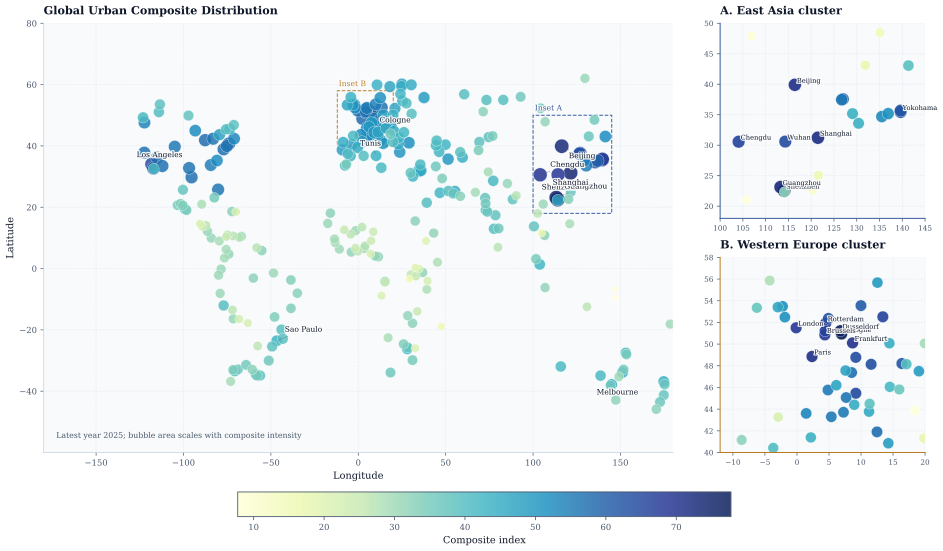
\includegraphics[width=0.96\textwidth]{submission_assets/Figure1_global_spatial_distribution.pdf}
  \caption{Latest-year city performance is geographically heterogeneous rather than clustered in a single world region. Insets improve readability in the densest East Asian and Western European clusters.}
  \label{fig:global_spatial_distribution}
\end{figure}
\FloatBarrier

\subsection{Measurement strategy}
The empirical design follows a simple principle: city outcomes should be read from city signals whenever possible, while broader macro series should remain contextual rather than masquerading as direct urban observations.
To make that distinction credible, city footprints are anchored to stable official polygons rather than point buffers, and directly observed urban signals remain separable from country-year controls.

\subsection{Data quality and comparability}
All sources pass through a common audit and harmonization step before entering the panel.
In the final sample, the objective row ratio, complete-city objective ratio, and verified row ratio are all 1.000, and policy-event entries retain auditable source references across 136 ISO3 codes.
The main limitation is that many macro indicators remain available only at the country-year level.
In the main specification we therefore avoid mechanical downscaling and keep those variables in the role of background context rather than direct city measurement.

\subsection{External measurement bridge}
To avoid relying only on internally constructed signals, we link the main transition diagnostics to independent external outcomes.
This bridge is corroborative rather than definitional: it does not replace the city-level outcome layer, but it tests whether the monitored states remain aligned with independently reported activity and output measures.
The bridge itself has two explicitly separate layers.
First, the paper uses observed city/metro-year GDP where it exists as the main external validation anchor.
Second, it reports a smaller set of country-year auxiliary endpoints as background consistency checks only.
These two layers are not interchangeable and are not interpreted as the same type of evidence.
Direct VIIRS signals now span the full panel and are incorporated as city-observed annual outcomes throughout.
The left-censored high-frequency channel is instead NO$_2$, which is observed from 2018 onward and therefore used only where actual coverage exists.
The nine auxiliary non-GDP endpoints are country-year World Bank series and are interpreted only as background consistency checks, not as independent city-year validation.

\subsection{Resolution hierarchy}
The empirical design follows a strict resolution hierarchy.
City-observed variables (urban structure, road-network dynamics, climate, and policy-event channels) are treated as the primary signal layer for transition-risk analysis.
Country-level macro variables are treated as supporting controls and are never interpreted as direct evidence of within-country micro measurement.
This separation prevents circular interpretation: transition claims rely on city-observed movement channels, while mixed-resolution variables absorb broad context rather than pretending to identify within-country city differences.
Appendix Table~\ref{tab:variable_credibility_appendix} inventories the core variables by resolution, coverage, and analytical role so that city-observed outcomes, mixed-resolution controls, and external-validation anchors remain visibly separated.

\subsection{Harmonization and uncertainty}
All sources are converted into a common annual city-year panel, tagged by source and resolution, and normalized within year where forward prediction would otherwise risk temporal leakage.
Missingness is handled with source-aware rules: macro variables are interpolated conservatively within country-year blocks, while city-level features are only filled when objective-source coverage remains intact.
The paper also separates measurement uncertainty from model uncertainty.
The former is addressed through auditing and conservative aggregation; the latter through out-of-time validation, OOD tests, and bootstrap or permutation inference.
This distinction matters because good fit does not guarantee clean interpretation, just as a significant coefficient does not guarantee transportable policy insight.

\subsection{Dashboard composite outcome}
For descriptive ranking and monitoring only, three sub-indices are constructed from normalized indicators:
\begin{equation}
  \Composite_{i,t} = w_E \cdot E_{i,t} + w_L \cdot L_{i,t} + w_I \cdot I_{i,t}.
\end{equation}

The baseline weights are $(w_E, w_L, w_I) = (0.45, 0.35, 0.20)$.
Following \citet{oecd2008handbook}, we conduct sensitivity analysis with four alternative schemes:\ PCA-derived weights, equal weights $(1/3, 1/3, 1/3)$, economic-heavy $(0.60, 0.25, 0.15)$, and innovation-heavy $(0.25, 0.30, 0.45)$.
Spearman rank correlations between baseline and alternatives are reported in Section~\ref{sec:robustness}.
This composite is used for composite ranking, transition visualization, and state benchmarking.
It is not admissible as the dependent variable in the main causal estimators, where only interpretable observed indicators are allowed.

\subsection{Dynamic transition variables}
For city $i$ and year $t$:
\begin{align}
  \Delta \Index_{i,t} &= \Index_{i,t} - \Index_{i,t-1}, \\
  \Delta^2 \Index_{i,t} &= \Delta \Index_{i,t} - \Delta \Index_{i,t-1}, \\
  \Volatility_{i,t} &= \mathrm{Std}(\Delta \Index_{i,t-2:t}).
\end{align}

Acceleration score:
\begin{equation}
  \AccScore_{i,t} = 100 \cdot \mathrm{MinMax}(0.55 \Delta \Index + 0.30 \Delta^2 \Index + 0.15 \text{Momentum}_2 - 0.22 \Volatility).
\end{equation}

Stall event (next period):
\begin{equation}
  \Stall_{i,t+1} = \mathbf{1}[\Delta \Index_{i,t+1} \le Q_{30}].
\end{equation}

In our sample, $Q_{30} = -0.508$ and the acceleration threshold $Q_{70} = 0.453$.
We verify robustness of stall classification by reporting performance metrics at $Q_{20}$ through $Q_{40}$ (Section~\ref{sec:robustness}).

%--- Methods subsections (continued from Data) ---

\subsection{Empirical strategy}
Empirically, the paper proceeds in three linked layers:
\begin{enumerate}[label=\arabic*.]
  \item \textbf{Monitoring layer:} Can city risk states be measured, externally bridged, and carried forward into out-of-time state classification, especially in first differences?
  \item \textbf{Dynamic-response layer:} Do policy-type event-study patterns reveal a fast-versus-slow temporal ordering in observed outcomes?
  \item \textbf{Spatial corroboration layer:} Do bounded spatiotemporal specifications support the interpretation that some responses diffuse beyond treated city boundaries?
\end{enumerate}

\subsection{Constructing fragile-boom states}
\paragraph{Risk prediction.} A candidate learner set (logit, tree ensembles, and boosting variants) predicts $\Stall_{i,t+1}$, outputting calibrated stall probability and a 0--100 risk score.
We compare several learners and select using out-of-time discrimination and calibration criteria.

\paragraph{Quadrant mapping.} Cities are mapped into interpretable states:\ \emph{accelerating}, \emph{steady}, \emph{fragile\_boom}, and \emph{recovery\_window}, using joint thresholds on acceleration and risk scores.

\paragraph{Archetype clustering.} DTW-based trajectory clustering with K-Medoids identifies long-run city archetypes:\ \emph{frontier\_accelerator}, \emph{resilient\_steady}, \emph{fragile\_rebound}, and \emph{structural\_stall}.

\subsection{State-classification protocol}
To prevent information leakage:
\begin{itemize}
  \item Dashboard target:\ $\Composite_{t+1}$ (one-step-ahead)
  \item Temporal split at 2022; evaluation on 2023--2025
  \item Leave-one-continent-out OOD tests for spatial generalization
  \item \textbf{Primary dynamic signal set:} city-observed time-varying channels (road-network evolution, OSM historical activity dynamics, climate variation, and policy-event flow/intensity).
  \item \textbf{First-difference two-track benchmark:} (A) raw $\Delta \Composite_{t \to t+1}$; (B) idiosyncratic residual $\Delta \Composite_{t \to t+1} - \mathbb{E}[\Delta \Composite_{t \to t+1}\mid\text{country, year}]$
  \item \textbf{Dynamic-feature filtering:} near-static predictors (identified by within-city temporal variation diagnostics) are excluded from difference benchmarking
  \item \textbf{Resolution-partitioned checks:} We compare city-observed feature tracks against mixed-resolution tracks (city outcomes + country-macro covariates) and treat disagreements as measurement-layer risk.
\end{itemize}

\subsection{Design-bounded causal diagnostics}
Primary causal outcomes are restricted to interpretable observed indicators (e.g., direct activity, physical-expansion, or knowledge/economic channels where observed).
Dashboard composites are excluded by design from the main causal outcome set.
The empirical anchor is the policy-type event study on observed fast and slow outcomes.
Multiple estimators with complementary assumptions are retained only to disclose design sensitivity around that central temporal pattern.
Appendix Table~\ref{tab:event_city_mapping_audit_appendix} makes the treatment layer auditable: direct-core cohorts are defined from explicit country-level registry events and then mapped to in-sample cities through a transparent country-year onset rule rather than through inferred within-country rollout dates.
In many cases these national policies are implemented through regionally concentrated urban programs, so the design is informative about shared policy timing while remaining weaker on within-country intensity heterogeneity.

\paragraph{Policy-type event study.} Dynamic treatment effects with relative-time indicators, implementing the heterogeneous-timing-robust specification of \citet{sun2021event}.

\paragraph{Auxiliary panel estimators.} Grouped DML-DID, DR-DID, and related panel estimators are used as auxiliary checks on local direction and design sensitivity rather than as the main empirical claim.

\paragraph{Pooled disclosure estimators.}
\textit{TWFE-DID baseline:}
\begin{equation}
  \mathit{Y}_{it} = \alpha_i + \gamma_t + \beta \mathit{D}_{it} + \theta' \mathit{X}_{it} + \varepsilon_{it},
\end{equation}
where $\mathit{D}_{it} = \text{treated}_i \times \text{post}_t$, with treatment defined from the policy event registry.

\textit{DR-DID:} Cross-fitted doubly robust DID on first differences, following \citet{santanna2020dr}.

\textit{Counterfactual checks:} Matrix completion \citep{athey2021matrix} and synthetic control \citep{abadie2010synthetic} are used only to bound interpretation around selected cases rather than to define the main estimand.

\subsection{Spatiotemporal causal model (Causal-ST)}
Causal-ST augments treatment analysis with:
\begin{itemize}
  \item Temporal lags of outcome and covariates
  \item Spatial lags based on KNN neighborhood structure
  \item Doubly robust estimation combining outcome regression and propensity weighting
\end{itemize}
Ablations systematically remove spatial controls, temporal controls, and the DR correction.

\subsection{Identification diagnostics protocol}
To keep causal interpretation disciplined, we run a structured diagnostics protocol before interpreting any ATT/CATE estimate.
\begin{enumerate}[label=\arabic*.]
  \item \textbf{Support diagnostics:} verify treated/control overlap in pre-treatment levels, trends, and key covariates.
  \item \textbf{Timing diagnostics:} inspect treatment cohort concentration and event-time support to avoid extrapolating sparse relative-time bins.
  \item \textbf{Pre-trend diagnostics:} report event-study lead coefficients, joint pre-period checks, and placebo-year distributions.
  \item \textbf{Estimator agreement diagnostics:} compare signs, orders of magnitude, and uncertainty bands across TWFE, DML-DID, DR-DID, Causal-ST, and counterfactual estimators.
  \item \textbf{Sensitivity diagnostics:} evaluate policy-source tracks, leave-one-continent stability, and multiple-testing-adjusted significance summaries.
\end{enumerate}

This protocol is designed to reduce two common failure modes in applied panel work:
over-interpreting one estimator in isolation, and post-hoc selection of favorable designs.
By committing to this fixed sequence, we treat disagreement across estimators as empirical information rather than as noise to be hidden.

%==============================================================================
\section{Results I: Fragile Boom, Temporal Mismatch, and External Validation}
\label{sec:forecast_results}
%==============================================================================

\subsection{Fragile boom as a measurable risk state}
Fragile boom is observable as a distinct high-acceleration, high-risk state rather than a narrative label.
In held-out data, the stall-state classifier reaches $\mathrm{ROC}$-$\mathrm{AUC}=0.742$, average precision $=0.474$, and Brier score $=0.203$, indicating non-trivial but bounded discrimination relative to static baselines.
The selected learner is \texttt{logit}, so the classification layer is comparatively parsimonious rather than a high-variance ensemble.
Longer-horizon classification weakens, which is why the paper uses this layer as forward-looking risk information rather than as the central empirical claim.

\textbf{Stall threshold sensitivity:} classification performance remains stable across alternative quantile thresholds (Q20--Q40), confirming that the stall-event definition is not driven by one cutoff.
The strongest classification features are recent growth, the observed physical stress signal, and medium-run regime-switching risk, suggesting that near-term transition dynamics dominate simple level-only covariates in event detection.
Latest-year quadrant distribution is: steady 48.14\%, fragile\_boom 24.41\%, recovery\_window 22.37\%, stalling 3.39\%, and accelerating 1.69\%.

\begin{figure}[H]
  \centering
  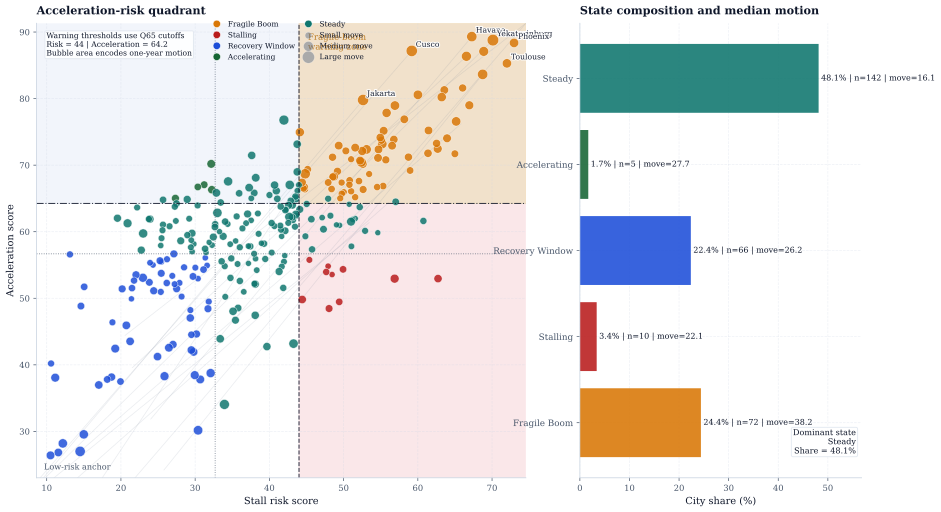
\includegraphics[width=0.90\textwidth]{submission_assets/Figure2_pulse_quadrant_scatter.pdf}
  \caption{Fragile-boom cities occupy a distinct high-acceleration, high-risk quadrant that static rankings cannot reveal. The upper-right shaded area denotes the forward-looking risk zone under quantile-calibrated thresholds.}
  \label{fig:quadrant_scatter}
\end{figure}
\FloatBarrier

\begin{figure}[H]
  \centering
  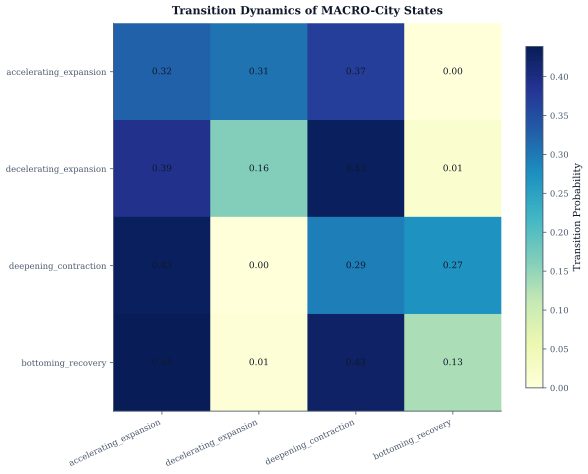
\includegraphics[width=0.90\textwidth]{submission_assets/Figure3_pulse_transition_heatmap.pdf}
  \caption{Most cities persist in place from one year to the next, but transition flows into fragile and recovery states remain economically meaningful. Diagonal dominance indicates persistence, while off-diagonal mass identifies recurrent regime-switch pathways.}
  \label{fig:transition_heatmap}
\end{figure}
\FloatBarrier

\subsection{Why observed city signals matter}
Figure~\ref{fig:observed_measurement_gain} makes the resolution hierarchy observable in the final panel rather than leaving it as a methodological claim.
In the current run, all rows are generated under the city-observed primary specification (share = 1.000), the mean number of directly observed channels per city-year is 5.23, and every row contains at least three directly observed channels and at least two dynamic channels.
Direct city-level macro observation is no longer zero: the observed city-macro row share is 0.215, while the fast NO$_2$ layer is directly observed for 72.7\% of city-year cells (2018--2025).
The remaining gaps are handled asymmetrically: unavailable channels are neutralized for causal work, while backcasted fast features are quarantined to prediction-only modules.
This rule prevents the main index and the main causal designs from reintroducing fabricated within-country variation through hidden imputations.

The source-group ablation reinforces this interpretation.
Relative to a macro-context-only specification, the observed-core feature block reduces RMSE from 3.460 to 1.172 for economic vitality, from 5.515 to 2.627 for livability, from 2.164 to 1.435 for innovation, and from 2.994 to 1.000 for the composite index.
Averaged across the four targets, the observed-core specification lowers RMSE by 1.975 points and raises $R^2$ by 0.350 relative to macro-context-only baselines.
Innovation remains the weakest target, but once policy context and the mixed full specification are added, the innovation gap narrows materially relative to the observed-core-only specification.

Cross-source consistency also remains non-trivial among the directly observed dynamic channels with real coverage.
Using road-growth intensity, OSM road growth, and OSM POI growth, the mean consistency score is 0.625, the high-consistency row share is 0.592, and the correlation between road-growth intensity and OSM road growth reaches 0.851 with perfect sign agreement.
The substantive point is not procedural but empirical:
the paper's main patterns are grounded in multiple directly observed city signals rather than in a purely macro-contextual construction.

\begin{figure}[H]
  \centering
  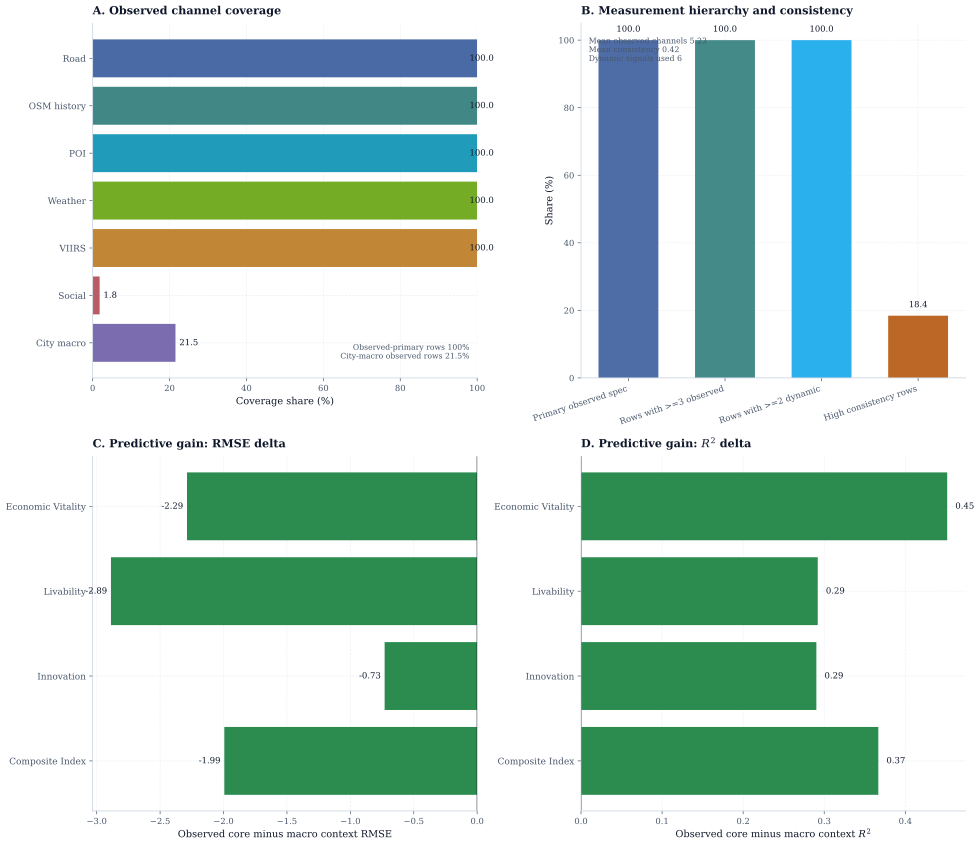
\includegraphics[width=0.96\textwidth]{submission_assets/Figure36_observed_measurement_gain.pdf}
  \caption{Observed city signals provide broader coverage and better empirical fit than macro-context-only inputs. The figure contrasts channel coverage, measurement hierarchy, and observed-core gains against macro-context baselines.}
  \label{fig:observed_measurement_gain}
\end{figure}
\FloatBarrier

\subsection{Bounded external validation}
A natural question is whether the monitored states map onto real city economic outcomes rather than remaining internal constructs.
This section addresses that question using only the city/metro-year observed GDP subset, not the country-year auxiliary endpoint layer reported later.
To answer it, we use the standardized subset of 89 OECD metropolitan areas with directly observed PPP GDP, yielding 749 city-year observations and 660 consecutive city-year pairs for forward validation.
This is a narrow external bridge rather than a global validation sample, and it constrains the paper most strongly in richer OECD metros.
The calibration evidence is intentionally presented in a restrained way.
Raw $\log(\mathrm{VIIRS\ NTL})$ is positively associated with observed PPP GDP, but only moderately so (pooled $R^2=0.103$, pooled Spearman $\rho=0.332$).
By contrast, the theory-anchored Cobb-Douglas vitality fit---which combines knowledge capital, built volume, and baseline population rather than using observed GDP directly---tracks observed PPP GDP much more closely (pooled $R^2=0.557$, pooled Spearman $\rho=0.755$).
For the argument of this paper, that is the more relevant bridge:
the vitality layer is not merely a monitoring construction, but a measurable proxy that co-moves with external metro-level output in a standardized sample.

We then ask a forward-looking question: does the dynamic risk layer help anticipate subsequent deterioration in real activity?
Defining an adverse outcome as bottom-quintile next-year observed PPP GDP growth, we evaluate rolling one-year-ahead ranking performance over test years 2020--2022.
A static-size baseline yields mean AUC 0.450, a volatility-only baseline yields 0.475, and a risk-only baseline reaches 0.640.
The fragile-boom indicator reaches mean AUC 0.646, while the joint risk-plus-acceleration specification reaches 0.668 and acceleration alone reaches 0.667.
The point is therefore not that the binary fragile-boom flag dominates every component baseline in pure ranking performance.
Rather, the concept preserves most of the gain from the richer dynamic score while remaining more interpretable than a continuous black-box risk index and clearly outperforming static size and volatility-only summaries.
The gain is not uniform in every year, and probability calibration remains modest, so we do not present this exercise as a long-horizon projection exercise.
The narrower conclusion is still important:
fragile-boom and related dynamic risk states contain forward-looking information about metro-level deterioration in this OECD subset that is not recoverable from static size alone.

\begin{table}[H]
\centering
\caption{Observed city/metro GDP validation bridge in the standardized OECD metro subset.}
\label{tab:gdp_validation_bridge}
\small
\setlength{\tabcolsep}{5pt}
\begin{tabular}{lrrr}
\toprule
Validation object & Sample & Metric & Value \\
\midrule
Raw VIIRS level $\rightarrow$ observed PPP GDP & 749 city-years & pooled $R^2$ & 0.103 \\
Cobb-Douglas vitality fit $\rightarrow$ observed PPP GDP & 749 city-years & pooled $R^2$ & 0.557 \\
Static size $\rightarrow$ next-year GDP slowdown & 2020--2022 rolling test & mean AUC & 0.450 \\
Volatility only $\rightarrow$ next-year GDP slowdown & 2020--2022 rolling test & mean AUC & 0.475 \\
Risk only $\rightarrow$ next-year GDP slowdown & 2020--2022 rolling test & mean AUC & 0.640 \\
Fragile-boom flag $\rightarrow$ next-year GDP slowdown & 2020--2022 rolling test & mean AUC & 0.646 \\
Acceleration only $\rightarrow$ next-year GDP slowdown & 2020--2022 rolling test & mean AUC & 0.667 \\
Risk + acceleration $\rightarrow$ next-year GDP slowdown & 2020--2022 rolling test & mean AUC & 0.668 \\
\bottomrule
\end{tabular}
\end{table}
\FloatBarrier

\begin{figure}[H]
  \centering
  \includegraphics[width=0.99\textwidth]{submission_assets/Figure37_gdp_validation_bridge.pdf}
  \caption{Observed PPP GDP provides an external anchor for the monitoring layer. The vitality fit tracks metro GDP in the standardized OECD subset, and dynamic risk states outperform static size, volatility-only, and risk-only baselines when ranking next-year GDP slowdowns.}
  \label{fig:gdp_validation_bridge}
\end{figure}
\FloatBarrier

\subsection{Supplementary dynamic diagnostics}
The paper's dynamic state layer is supplementary rather than central.
For slow-moving level outcomes such as $\log(\mathrm{VIIRS\ NTL})_{t+1}$, performance is strong mainly because persistence is strong: linear regression and Extra Trees both remain close to the persistence frontier, and cross-continent OOD error is similarly low.
The more informative test is the stricter difference benchmark.\label{sec:fd_regression_failure}
There, raw annual changes remain near the random-walk frontier, whereas idiosyncratic differences become modestly positive once common country-year shifts are removed (best $R^2=0.067$).
The implication is limited but useful: fast variables help recover some city-specific short-run variation, yet short-horizon turning points remain substantially harder to predict than medium-run temporal mismatch.
The NO$_2$ backcast module contributes 885 early-sample rows to this supplementary track while remaining excluded from all main causal outcome specifications.

\begin{figure}[H]
  \centering
  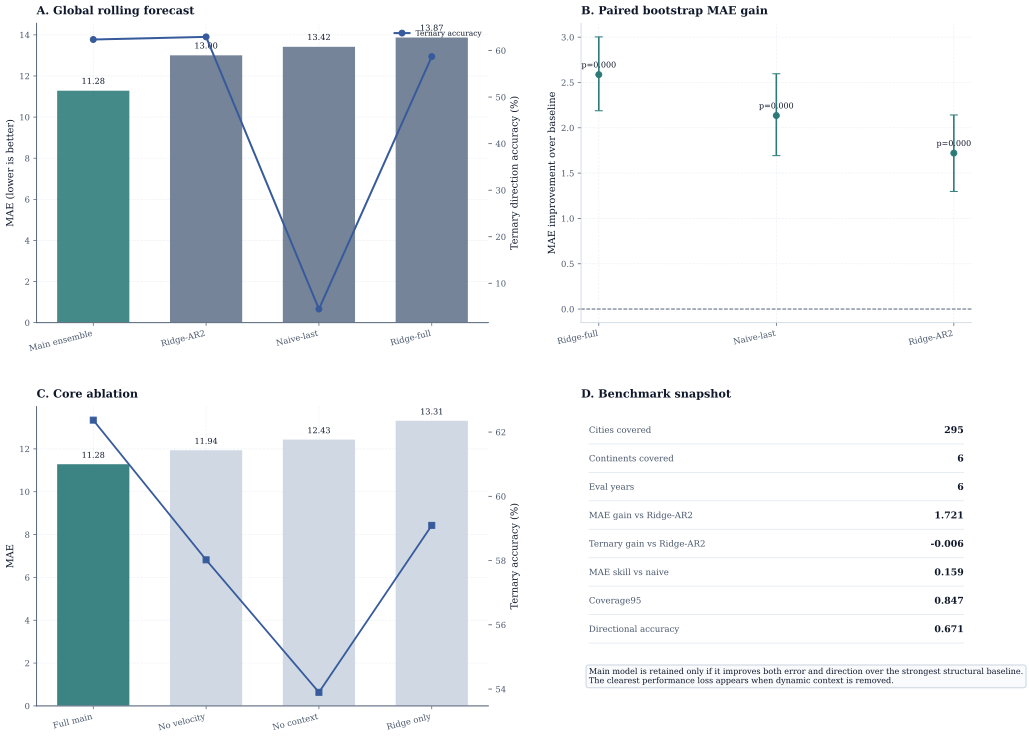
\includegraphics[width=0.96\textwidth]{submission_assets/Figure33_dynamic_method_core_benchmark.pdf}
  \caption{A supplementary benchmark showing why the paper does not rely on short-horizon dynamic projection as its central claim. Persistence remains strong in levels, while transition-direction gains remain limited even when dynamic features improve absolute error.}
  \label{fig:dynamic_method_core}
\end{figure}
\FloatBarrier

The stricter delta-first rolling benchmark in Figure~\ref{fig:dynamic_method_core} reinforces this conclusion.
When the target is defined as direct one-step change rather than level extrapolation, the main dynamic model attains MAE $=11.284$, RMSE $=14.314$, and ternary accuracy $=0.624$.
Relative to a strong ridge-AR(2) baseline, this yields a 1.721-point MAE improvement, although ternary accuracy is statistically indistinguishable in this run ($p=0.694$).
The appropriate reading is therefore narrow.
The dynamic layer improves absolute error relative to a strong baseline, but it does not yet deliver a stable directional advantage.
These benchmarks are retained as calibration checks rather than as a separate methodological contribution.

%==============================================================================
\section{Results II: Policy Timing Diagnostics and Spatial Stress Tests}
\label{sec:causal_results}
%==============================================================================

\subsection{Policy-type timing diagnostics under audited policy timing}
\begin{figure}[H]
  \centering
  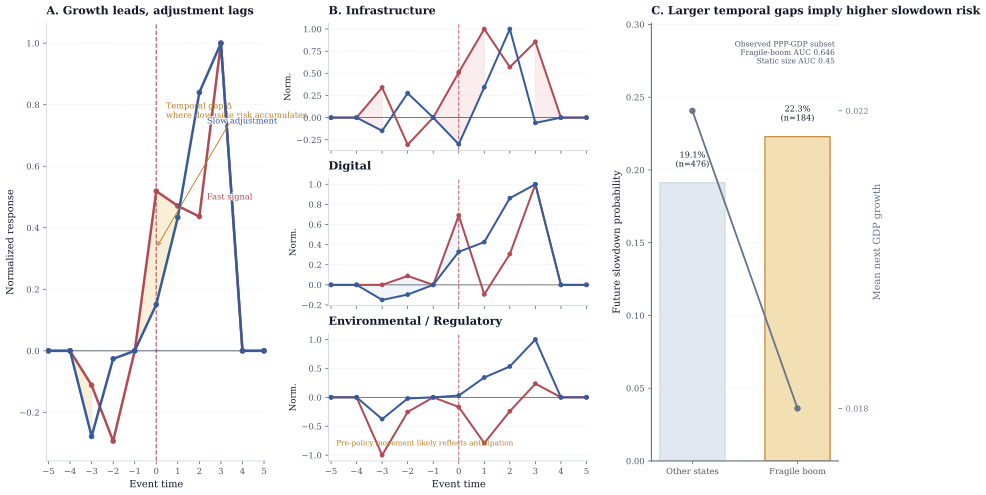
\includegraphics[width=0.99\textwidth]{submission_assets/Figure4_event_study_dynamic_effects.pdf}
  \caption{Design-bounded timing diagnostics. Panel A summarizes fast versus slow monitored responses around audited policy timing. Panel B shows how those timing patterns differ across infrastructure, digital, and environmental/regulatory interventions. Panel C links fragile-boom states to subsequent metropolitan GDP slowdown in the observed-GDP subset.}
  \label{fig:event_study_dynamic}
\end{figure}
\FloatBarrier

Figure~\ref{fig:event_study_dynamic} is best read as a timing summary rather than as a decisive causal figure.
Panels A and B organize the paper's central timing evidence: fast monitored signals can move earlier than slow adjustment proxies, but the strength and credibility of that pattern vary by policy bucket.
Panel C closes the loop by linking fragile-boom states to subsequent metropolitan GDP slowdown in the observed-GDP subset.
For the fast outcome, the main specification uses observed NO$_2$ only (2018--2025), sacrificing the early panel in exchange for a cleaner outcome definition.
Throughout, we interpret NO$_2$ as a fast-moving indicator of human activity and combustion intensity, complementary to slower measures of urban adjustment rather than a sufficient summary of the urban economy on its own.

Three policy-type response patterns stand out, and together they support the paper's central claim that policy effects are temporally ordered rather than well summarized by one pooled coefficient.
Infrastructure treatment shows the clearest short-run tension: the slow-response profile is negative, while the fast NO$_2$ panel exhibits a weak positive pulse around event time $t=0$ to $t=3$.
Digital policy barely moves fast NO$_2$, but its slow VIIRS response turns positive after two to three years, consistent with delayed diffusion of digital investment into visible urban activity.
Environmental and regulatory interventions occupy a third pattern, with a non-trivial fast-panel pre-trend diagnostic ($p=0.032$) that is more plausibly read as anticipation and compliance timing.

Taken together, these panels show that policy timing differences are systematic even though their exact causal interpretation remains bounded by aggregated policy onset and residual within-country heterogeneity.
Dose-response evidence remains limited, and the continuous-dose DID estimate is small and statistically weak.
We therefore treat policy type and response timing as evidence about temporally ordered urban adjustment under audited policy timing, while reserving finer-grained rollout claims for richer assignment data.
Appendix Table~\ref{tab:mechanism_proxy_appendix} adds supplementary proxy-consistency checks.
Infrastructure combines a weak positive fast NO$_2$ pulse with a negative local road-adjustment proxy, pointing to near-field disruption rather than immediate capacity gains.
Digital treatment shows delayed slow-variable gains and a weakly positive built-surface catch-up proxy, while environmental/regulatory episodes continue to show their clearest signal in anticipation-sensitive fast-channel diagnostics rather than contemporaneous level shifts.

\subsection{Estimator disclosure: pooled average effects are unstable}
\textbf{Key finding:} pooled estimates remain design-sensitive even after the treatment definition is tightened, and they should be read as country-year timing contrasts rather than fully city-specific ATT estimates.
Across multiple estimators with complementary assumptions, some pooled specifications are mildly positive, some are near zero, and some remain negative.
We therefore do not interpret any single pooled coefficient as definitive.
Instead, estimator disagreement is informative in its own right: once timing heterogeneity, local congestion costs, and cross-city spillovers are allowed to matter, a single global average becomes an unstable summary of urban policy response.
Appendix Table~\ref{tab:core_causal_disclosure_appendix} reports the full pooled-estimator disclosure table.

\subsection{Heterogeneity matters more than the pooled average}
The practical implication of a narrowed but still design-sensitive pooled ATT is not ``no policy matters''; it is ``average effects remain a poor summary when treatment bundles and local conditions differ sharply.''
In our data, treatment timing, intensity, and baseline resilience vary across continents and city archetypes.
When such heterogeneity is large, averaging can still obscure offsetting positive and negative responses, even after tightening the treatment definition.
This is precisely the setting where design triangulation and subgroup diagnostics are necessary.

We therefore treat pooled estimates as a first-pass diagnostic and then shift to three heterogeneity lenses:
(i) geographic heterogeneity (continent-level CATE),
(ii) trajectory-regime heterogeneity (fragile vs resilient clusters),
and (iii) policy-source heterogeneity (external direct vs sensitivity tracks).
Because treatment timing is still assigned at the country-year level, these heterogeneity patterns are descriptive segmentation tools rather than standalone causal CATE claims.
The consistency of the fragile-boom signal across these lenses is more informative for governance than any single global ATT.
This same heterogeneity explains why pooled and localized estimates need not move together.
The pooled DID estimand averages across cities, years, and treatment cohorts; once treatment intensity, baseline development stage, and spillover exposure differ sharply, positive and negative local responses can offset in the aggregate.
For that reason, weak pooled coefficients are most informative as a global constraint, while subgroup and spatiotemporal estimates are more informative about where local congestion costs and broader network benefits are concentrated.

\subsection{Spatial corroboration}
Causal-ST provides suggestive but non-decisive positive localized effects.
In the fully adjusted ablation row, the distance-based specification recovers ATT $=0.051$ with a percentile bootstrap 95\% confidence interval of [0.004, 0.084].
The companion two-sided bootstrap sign $p$-value is 0.10, so we treat the localized positive sign as supportive but not dispositive.
Its substantive value lies less in the headline magnitude than in the topology comparison itself.
Ablations reveal:
\begin{itemize}
  \item No spatial controls: ATT = 0.043
  \item No temporal controls: ATT = 0.046
  \item Flight-network spatial weights: ATT = 0.040
  \item Plugin without DR: ATT = 0.054
\end{itemize}

The central point is that the sign of the spatially adjusted estimate remains positive under both geographic and flight-network topologies.
The flight-based estimate is slightly smaller, but it does not reverse direction.
This supports a two-channel interpretation of spillovers:
policy effects diffuse through physical neighborhood structure and through long-range connectivity in the global mobility network \citep{redding2017quantitative}.
The main text uses KNN geography and flight connectivity because those matrices remain globally comparable across the full 295-city sample.
As an appendix robustness, we replace the geographic KNN map with a road-structure accessibility proxy derived from cleaned OSM road attributes and continent-bounded distance corridors.
Under that specification, the global Causal-ST estimate remains positive at 0.052 with a 95\% confidence interval of [$-0.002$, 0.088].
Appendix Table~\ref{tab:road_proxy_appendix} reports the full set of road-proxy estimates, including continent-specific results and a dense-core Europe/North America specification.
That dense-core specification tilts slightly negative, which is substantively useful rather than contradictory: once topology is forced toward high-density continental road corridors, the estimand shifts toward near-field congestion and construction frictions rather than broader long-range spillovers.
Read together with the policy-type results, the pattern is economically intuitive.
Infrastructure episodes can impose local short-run costs---construction frictions, congestion, resource diversion---that show up as weak or negative local slow-variable responses.
At the same time, the spatially augmented Causal-ST estimand remains positive, indicating that broader network benefits are not exhausted by the local city boundary.
Conventional pooled estimators are therefore not simply ``wrong''; rather, they average local cost and network benefit into a diluted coefficient.
The contribution of the spatiotemporal design is to show that these mechanisms can coexist instead of being forced into a single universal scalar ATT, while still stopping short of a strong city-level causal claim.

\begin{figure}[H]
  \centering
  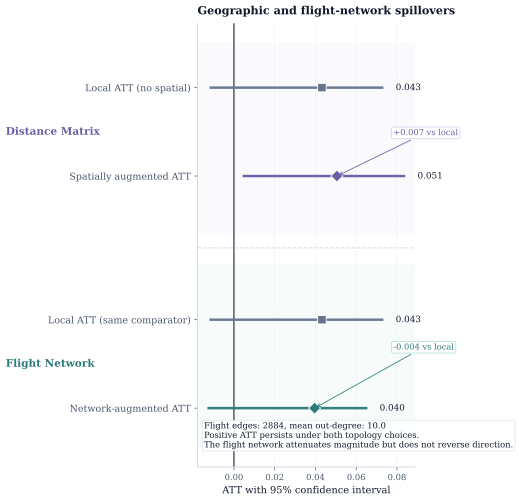
\includegraphics[width=0.97\textwidth]{submission_assets/Figure5_causal_st_dynamic_att.pdf}
  \caption{Spatially augmented effects remain positive under both geographic and flight-network topologies, even when local average effects are modest. The forest plot contrasts local and spillover-aware estimates under both network constructions.}
  \label{fig:causal_st_dynamic}
\end{figure}
\FloatBarrier

\subsection{Auxiliary country-year endpoints}
This section is intentionally separate from the observed-GDP bridge above.
All nine series reported here are country-year endpoints, so they serve only as background consistency checks and not as city-level ranking or validation targets.
Nine auxiliary external outcomes are evaluated on a country-year panel rather than a city-year panel: the average absolute TWFE statistic is $|t|=0.971$.
The strongest signal appears in PM$_{2.5}$ exposure ($t=-3.290$, $p=0.001$, within-family BH $q=0.009$).
Fixed broadband subscriptions are directionally positive at the raw-test level ($t=1.964$, $p=0.0495$) but do not survive within-family multiplicity correction, while the combined electricity--broadband activity proxy is statistically weak ($t=0.479$, $p=0.632$).
These are background annual endpoint tests rather than decisive cross-domain confirmations.
We therefore interpret the external layer as bounded country-year consistency evidence rather than as independent city-level validation.
Observed metropolitan GDP remains the harder external anchor: panel-wide VIIRS coverage is now complete, but luminosity is still an indirect proxy for economic output.

\subsection{Practical effect-size interpretation}
To reduce ambiguity between statistical and policy significance, we report effect sizes in decision terms.
For state-classification modules, the key question is not whether AUC is ``high'' in isolation, but whether risk ranking improves intervention targeting relative to static-score baselines.
For causal modules, the key question is not whether one estimator yields the largest coefficient, but whether directional conclusions persist across credible design perturbations.

Under this lens, three practical conclusions are stable:
\begin{enumerate}[label=(\roman*)]
  \item pooled average treatment effects are too small and unstable for one-size-fits-all policy prescriptions;
  \item heterogeneity by continent and regime is large enough to justify segmented policy menus;
  \item fragile-boom monitoring provides incremental forward-looking risk information beyond static composite rankings.
\end{enumerate}

These conclusions remain valid even when absolute magnitudes differ across estimators.
Hence the manuscript emphasizes robust qualitative patterns and transparent uncertainty reporting, rather than over-optimizing one preferred numeric estimate.

%--- Heterogeneity and Mechanisms (subsection of Causal Diagnostics) ---
\subsection{Heterogeneity and Mechanisms}
\label{sec:heterogeneity}

Causal-ST CATE by continent reveals pronounced heterogeneity:
\begin{table}[H]
\centering
\caption{Policy responses differ sharply across continents rather than collapsing to a single global treatment effect.}
\label{tab:cate_continent}
\begin{tabular}{lrr}
\toprule
Continent & CATE & $N$ \\
\midrule
Africa & $+0.198$ & 572 \\
Asia & $-0.026$ & 814 \\
Europe & $-0.193$ & 737 \\
North America & $-0.451$ & 484 \\
Oceania & $-0.070$ & 209 \\
South America & $+0.096$ & 429 \\
\bottomrule
\end{tabular}
\end{table}
\FloatBarrier

The pattern remains asymmetric: North America and Europe are more negative, while Africa and South America are modestly positive and Asia is near zero.
This split is consistent with baseline-dependent treatment response and supports segmented policy interpretation rather than global averaging.

In the latest year, the global pulse-state mix remains non-trivial in the high-risk zone: fragile\_boom accounts for 24.41\% of cities (steady 48.14\%, recovery\_window 22.37\%, stalling 3.39\%, accelerating 1.69\%).
This pattern suggests that short-run acceleration and elevated downside risk can co-exist in a materially large share of cities that static level rankings do not reveal.

\begin{figure}[H]
  \centering
  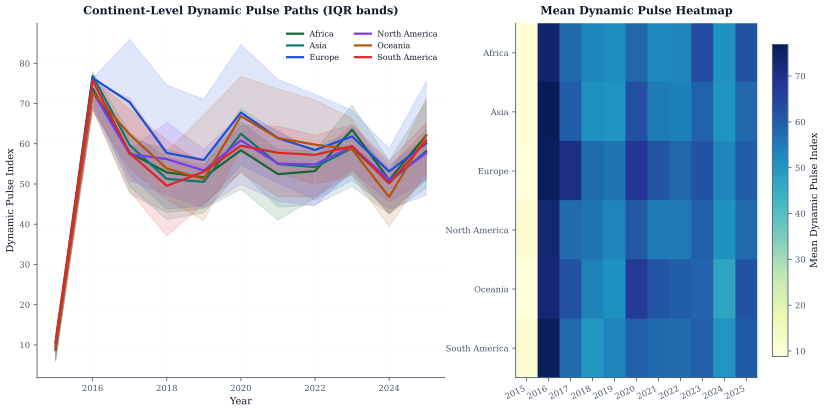
\includegraphics[width=0.90\textwidth]{submission_assets/Figure13_dynamic_pulse_continent_evolution.pdf}
  \caption{Fragile-boom and recovery states evolve differently across regions, reinforcing the importance of heterogeneity over global averaging. The figure complements point estimates with temporal distributional dynamics.}
  \label{fig:continent_pulse_evolution}
\end{figure}
\FloatBarrier

%==============================================================================
\section{Robustness and Limitations}
\label{sec:robustness}
%==============================================================================

\subsection{Sensitivity to state definitions and timing cutoffs}
The main monitoring results are stable to reasonable alternatives in both weighting and threshold design.
Dashboard rankings remain highly correlated across PCA-derived, equal, economic-heavy, and innovation-heavy weights \citep{oecd2008handbook,nardo2005tools}, while stall-risk classification remains broadly similar across $Q_{20}$ to $Q_{40}$ cutoffs.
Likewise, the fragile-boom zone remains non-trivial under alternative joint thresholds for risk and acceleration, indicating that the state is not an artifact of one plotting convention.

\subsection{Timing diagnostics and design sensitivity}
The timing diagnostics are mixed rather than uniformly reassuring.
Within the policy-type panels, the fast environmental/regulatory NO$_2$ series shows the clearest anticipation pattern ($p=0.032$), while infrastructure and digital panels are more stable.
At the aggregate staggered-design level, the updated unique-geometry pretrend gate now passes for the main design, but it does so under a short pre-period with only three lead points and therefore should not be over-read as a blanket endorsement of pooled DID geometry.
That omnibus gate still pools heterogeneous policy clocks and remains more conservative than any one policy-type panel.
The evidence is therefore stronger on qualitative timing differences within the policy-type panels than on any blanket claim that the broader staggered envelope is clean in every design dimension.
Placebo, bootstrap, and leave-one-continent-out checks lead to the same practical conclusion: the paper's core qualitative claims are more stable at the level of timing patterns than at the level of any one pooled coefficient.

\begin{figure}[H]
  \centering
  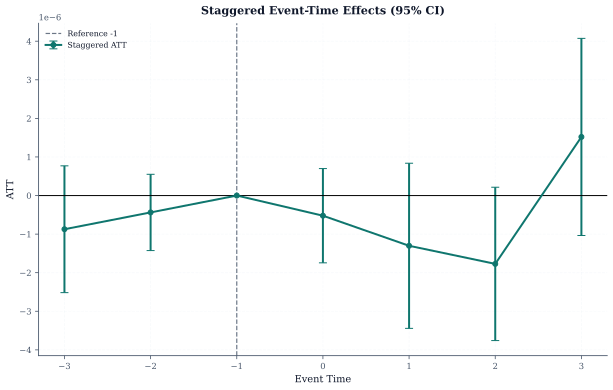
\includegraphics[width=0.90\textwidth]{submission_assets/Figure6_staggered_event_effects.pdf}
  \caption{Staggered event-study estimates remain informative about timing geometry. The updated unique-geometry pretrend check passes for the main design, but uncertainty widens away from treatment and pooled geometry remains more fragile than the policy-type timing panels. Dynamic coefficients and confidence bands are reported under heterogeneous adoption timing.}
  \label{fig:staggered_event_effects}
\end{figure}
\FloatBarrier

Across the broader robustness envelope---including family-specific multiple-testing correction, alternative policy-source tracks, event-time windows, continent leave-one-out subsets, and estimator families---the main patterns remain more stable in direction than in exact magnitude.
That is why the paper emphasizes temporal ordering, heterogeneity, and externally anchored risk states rather than insisting on one global treatment parameter.

%==============================================================================
\section{Discussion}
\label{sec:discussion}
%==============================================================================

\subsection{The fragile-boom concept and its broader significance}
The coexistence of acceleration and elevated stall risk in nearly one-fifth of sampled cities challenges a foundational assumption of urban policy: that growth, once visible, is self-sustaining.
We propose three channels through which fragile booms arise:
(i)~front-loaded investment with delayed productivity realization;
(ii)~structural transition frictions, including sectoral reallocation costs; and
(iii)~rigid factor markets that amplify volatility during demand shocks.
Crucially, fragile boom is not a synonym for volatility.
In the observed-GDP subset, a volatility-only baseline performs poorly relative to the fragile-boom state and the joint risk-plus-acceleration track.
What the concept adds is a \emph{conjunctive} interpretation: growth remains visible precisely when adjustment persistently lags, so risk is temporally structured rather than generically unstable.

This pattern connects directly to the middle-income-trap literature \citep{hausmann2005growth,eichengreen2012slowdown}.
At the national level, trap dynamics arise when early growth drivers are exhausted before productivity institutions are upgraded.
Fragile boom can be understood as the city-level analogue: visible acceleration persists while structural adjustment lags and cumulative downside risk builds underneath.
This interpretation bridges macro development theory and place-based urban diagnostics.

\subsection{Why timing matters more than any single estimator}
The main contribution of the paper is not that one estimator defeats another, but that the timing structure of urban adjustment becomes visible once fast and slow margins are studied jointly.
Prediction alone can rank near-term risk but cannot explain why trajectories diverge.
Pooled causal estimates, by contrast, become unstable when treatment bundles and local conditions differ sharply.
Taken together, the two layers point to a narrower substantive conclusion: cities appear more fragile when visible expansion outruns slower adjustment, and this monitored mismatch is more informative than any single average effect currently available from the policy layer.

\subsection{Implications for urban governance}
These findings suggest three shifts in urban policy practice.
First, governance should track velocity and volatility rather than levels alone, because static rankings cannot reveal fragile-boom states.
Second, resilience investments should be front-loaded during growth phases rather than deployed reactively after crises.
Third, interventions should be tailored to continent and development-stage heterogeneity, since pooled average effects are too unstable to guide one-size-fits-all prescriptions.

In practical terms, agencies can attach a dynamic monitoring layer to existing scorecards: track acceleration, stall risk, and uncertainty bands; monitor whether fast-flow and slow-stock signals move in the same direction; and treat divergence as forward-looking risk information rather than as a final policy verdict.
The central institutional gain is earlier detection of ``acceleration with hidden fragility,'' enabling preventive diagnosis before stall events materialize.

%--- Limitations (subsection of Robustness and Limitations) ---
\subsection{Limitations}

\begin{enumerate}
  \item \textbf{Treatment endogeneity and assignment scale:} Policy event timing is identified from registry data rather than randomized experiments, and audited direct-core events are anchored to registry-dated policy onset. Many of these policies are implemented through regionally concentrated urban programs, but within-country rollout intensity is still only partially observed.
  \item \textbf{City-level macro coverage remains partial:} The main specification now disables deterministic country-to-city macro disaggregation, but many macro fields still exist only at country-year resolution. A next step is to incorporate sub-national state/province accounts and formal downscaling layers where administrative coverage permits, so that macro context can be measured closer to the city-year outcome scale.
  \item \textbf{Cross-level predictability constraint:} A subset of controls remains at country-year resolution, while outcomes are city-year. Although the idiosyncratic first-difference track is now positive under city-observed feature prioritization, the raw-difference track remains difficult, and this resolution gap still limits micro-dynamic interpretability for macro channels.
  \item \textbf{External validity remains narrow:} Observed metropolitan PPP GDP is available only for the standardized OECD subset, while the nine auxiliary annual external outcomes are country-year rather than city-year series. A broader validation set would benefit less from additional satellite-light coverage---which now spans the panel---than from richer direct metro output, employment, and firm-demography series.
  \item \textbf{Forward-looking risk information is supplementary rather than central:} The main held-out stall classifier reaches $\mathrm{ROC}$-$\mathrm{AUC}=0.742$, but multi-horizon strength falls into the mid-0.6 range and the short-horizon nowcast direction test remains near chance. This layer is therefore used as forward-looking risk information rather than as a deployable forecasting claim.
  \item \textbf{Mechanism evidence remains proxy-based:} The paper triangulates NO$_2$, VIIRS, road evolution, and policy-specific timing patterns, but it does not claim a fully identified mediation analysis for investment timing, congestion, or factor rigidity channels. In this setting, NO$_2$ is used as a fast-moving indicator of combustion-linked human activity rather than as a sufficient stand-alone summary of broader urban performance.
  \item \textbf{Composite weights:} While sensitivity analysis shows robustness, the baseline weights remain expert-elicited rather than derived from a formal optimization or stakeholder process.
  \item \textbf{Short panel and slow variables:} Eleven years (2015--2025) limits the power of pre-trend tests and long-horizon dynamics analysis, especially for slow-moving urban form channels such as VIIRS and built environment stocks. For that reason, the paper interprets remote-sensing levels jointly with richer micro-geographic POI and road-evolution channels, which provide a complementary middle-speed view of structural change.
  \item \textbf{Spatial topology remains incomplete:} The present spillover analysis now includes an appendix road-structure accessibility proxy derived from cleaned OSM road attributes, and that robustness preserves a positive global sign while remaining heterogeneous across continents. What remains missing is a fully global route-time or shortest-path matrix built from realized transport networks.
\end{enumerate}

The main next-step priorities are narrower rather than broader: a frozen single analysis version with synchronized text and assets, city-specific within-country rollout evidence beyond the audited country-year mapping in Appendix Table~\ref{tab:event_city_mapping_audit_appendix}, more sub-national macro coverage where official series exist, and transport-accessibility matrices based on realized route times rather than road-structure proxies alone.

\subsection{Interpretive boundaries}
The main identification risks remain endogenous timing, short pre-period support for some cohorts, possible spillover misspecification, and the partial coexistence of city-year outcomes with country-year macro controls.
Appendix Table~\ref{tab:threat_matrix_appendix} reports these threats in full.
At the level of substantive interpretation, current evidence supports the following:
\begin{enumerate}
  \item reproducible objective-source data construction and transition diagnostics;
  \item non-trivial but geographically narrow external calibration of the monitored vitality/risk layer against observed metropolitan GDP;
  \item empirical prevalence of fragile-boom states in the audited panel;
  \item suggestive policy-timing heterogeneity across buckets and geographies under audited policy timing.
\end{enumerate}

Current evidence does \emph{not} support:
\begin{enumerate}
  \item a universal positive average treatment effect across all cities;
  \item fully city-specific ATT/CATE interpretations under the current treatment mapping;
  \item treating country-year auxiliary endpoints as independent city-level external validation;
  \item treating NO$_2$ movement as a sufficient stand-alone summary of overall urban performance;
  \item mechanical policy optimization from the current evidence alone.
\end{enumerate}
Those boundaries are integral to the argument rather than peripheral caveats: the paper is about temporally structured urban fragility, not about extracting a single universal treatment coefficient.

%==============================================================================
% Section 12 (Policy Translation and Deployment Protocol) removed per revision.
%==============================================================================

\section{Conclusions}

This paper began with a simple puzzle: why do some cities continue to look successful even as the conditions for slowdown are already forming?
The answer advanced here is that urban growth is temporally uneven.
Fast margins of expansion respond first, slower structural margins respond later, and the interval between them is precisely where fragility accumulates.

The main result is that urban adjustment is temporally asymmetric: fast margins of expansion respond earlier than slower structural margins, and the gap between them is where fragile-boom risk accumulates.
Across the paper's evidence tiers, that pattern is more stable than any single pooled coefficient.
\emph{Fragile boom} can be measured as a distinct urban risk state, policy responses differ systematically by type and timing, and in a limited OECD metro subset these states carry forward-looking information about subsequent GDP slowdown.
The policy layer is more constrained.
Aggregated policy timing, design-sensitive pooled estimators, and short pre-period support mean that the current evidence is stronger on temporal ordering than on universal city-level ATT claims about how policy reshapes urban adjustment.

The broader implication is narrower than a universal policy law but stronger than a static descriptive scorecard.
Urban fragility is not simply the absence of growth; it is a monitored state in which visible expansion and slower adjustment fall out of sync.
By formalizing \emph{fragile boom} in that bounded way, the paper argues for a shift away from static scorecards and toward a more temporally grounded account of urban growth, while making explicit where stronger rollout data and cleaner identification are still required.

%==============================================================================
% References
%==============================================================================

\appendix
\section{Appendix: Backcasted NO$_2$ Robustness}
\label{app:no2_backcast}

The main fast-variable specification uses observed NO$_2$ only and therefore restricts the causal sample to 2018--2025.
To check whether the core interpretation is mechanically driven by left-censoring of the early panel, we estimate an appendix-only robustness design in which NO$_2$ is backcasted for 2015--2017 using predictors observed no later than 2023.
These backcasted features never enter the main causal outcome specification.
They are used only as a robustness expansion of the sample window.

\begin{table}[H]
\centering
\caption{Appendix Table A1. Backcasted NO$_2$ does not overturn the main fast-variable ordering in the full-sample robustness design (2015--2025).}
\label{tab:no2_backcast_appendix}
\small
\setlength{\tabcolsep}{5pt}
\begin{tabular}{lrrrrr}
\toprule
Policy bucket & DML coef ($\times 10^{-6}$) & $p$-value & Mean post coef ($\times 10^{-6}$) & Pretrend $p$ & Filled rows \\
\midrule
Infrastructure & 0.757 & 0.103 & 4.708 & 0.245 & 885 \\
Digital & 0.253 & 0.587 & 2.453 & 0.408 & 885 \\
Environmental / regulatory & 0.029 & 0.958 & -0.519 & 0.406 & 885 \\
\bottomrule
\end{tabular}
\end{table}
\FloatBarrier

Table~\ref{tab:no2_backcast_appendix} does not overturn the main fast-variable story.
Infrastructure remains the only bucket with a visibly positive short-run NO$_2$ pulse, while digital and environmental/regulatory treatments remain close to zero once uncertainty is acknowledged.
In that narrower sense, the substantive ordering is stable to sample expansion, even though the appendix specification is intentionally treated as secondary evidence.

\section{Appendix: Pooled-estimator disclosure}
\label{app:pooled_disclosure}

\begin{table}[H]
\centering
\caption{Appendix Table A2. Global average policy effects remain design-sensitive even after treatment tightening to the direct-core track.}
\label{tab:core_causal_disclosure_appendix}
\small
\setlength{\tabcolsep}{5pt}
\begin{tabular}{lrrrrrr}
\toprule
Method & Estimate & SE & 95\% CI & $t$-stat & Bootstrap sign $p$ & $N$ \\
\midrule
TWFE-DID & 0.060 & 0.040 & [$-0.019$, 0.139] & 1.488 & 0.140 & 935 \\
Staggered DID & 0.063 & -- & [$-0.011$, 0.136] & 1.678 & 0.193 & 935 \\
DML-DID & $-0.189$ & 0.062 & [$-0.311$, $-0.068$] & $-3.048$ & 0.003 & 934 \\
DR-DID & 0.014 & 0.012 & [$-0.010$, 0.039] & 1.152 & 0.302 & 836 \\
Causal-ST & 0.051 & 0.024 & [0.004, 0.084] & 2.094 & 0.100 & 3245 \\
\bottomrule
\end{tabular}
\end{table}
\FloatBarrier
\noindent\textit{Notes:} The main outcome is $\log(\mathrm{VIIRS\ NTL})$ and the main treatment is the direct-core policy track. Staggered DID reports its published confidence interval directly. Causal-ST reports a percentile bootstrap confidence interval together with a two-sided sign-bootstrap $p$-value from 60 successful draws, so the two uncertainty summaries need not line up exactly.

\section{Appendix: Supplementary counterfactual and effect envelope}
\label{app:counterfactual_envelope}

Synthetic control for the treated Ireland case reports a positive post-treatment gap of 0.526, whereas panel-wide Causal-ST reports a much smaller positive average ATT of 0.051.
This gap is not contradictory.
It reflects the difference between a one-case long-horizon counterfactual and a pooled spatiotemporal panel estimand.
We therefore avoid collapsing these magnitudes into one policy number and instead use them to define a conservative effect envelope for decision interpretation.

We summarize the remaining model dependence with a signed effect envelope rather than treating any one estimator as the final word:
\[
\mathcal{E}_{\text{signed}} = \left[\min\{0.060, 0.063, -0.189, 0.014, 0.051, 0.526\},\ \max\{0.060, 0.063, -0.189, 0.014, 0.051, 0.526\}\right] = [-0.189, 0.526].
\]
The purpose of this envelope is modest.
It communicates model-dependence risk and prevents over-confidence in any single functional-form assumption.
The remaining fragility lies in heterogeneous timing, policy bundling, and topology choice, not in one mechanical pooled sign reversal.

\begin{figure}[H]
  \centering
  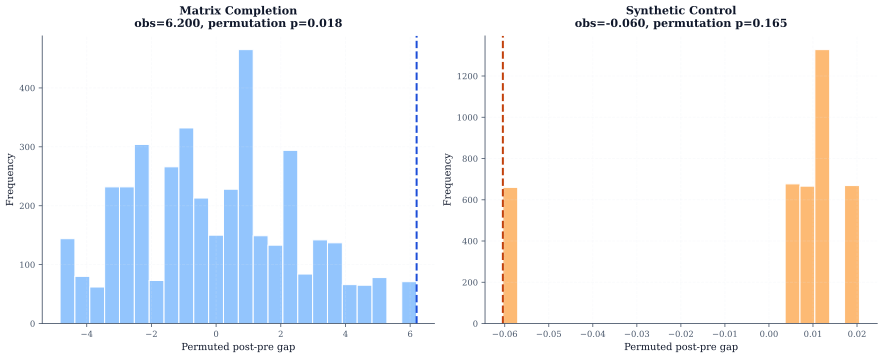
\includegraphics[width=0.90\textwidth]{submission_assets/Figure34_nonse_permutation_distribution.pdf}
  \caption{Appendix Figure A1. Design-dependent estimators still produce interpretable effect envelopes once uncertainty is reported transparently. Dashed lines denote the observed post-pre gap statistics against their permutation distributions.}
  \label{fig:nonse_permutation}
\end{figure}
\FloatBarrier

\section{Appendix: Identification Risks and Mitigation}
\label{app:threat_matrix}

\begin{table}[H]
\centering
\caption{Appendix Table A3. The main identification risks are explicit, partially mitigated, and still consequential for claim boundaries.}
\label{tab:threat_matrix_appendix}
\small
\setlength{\tabcolsep}{4pt}
\begin{tabular}{p{0.21\textwidth}p{0.27\textwidth}p{0.24\textwidth}p{0.20\textwidth}}
\toprule
Threat & Why it matters & Current mitigation & Remaining risk \\
\midrule
Endogenous timing & Adoption can correlate with latent trends & External-direct event track, pretrend tests, placebo timing checks & Event timing granularity remains limited \\
Differential trends & Treated/control drift may differ pre-treatment & TWFE, event-study, and DML triangulation & Short pre-period for some cohorts \\
Spillovers & Neighbor interventions contaminate controls & Causal-ST spatial controls and ablations & Network misspecification possible \\
Measurement heterogeneity & Country-level macro available for part of control set & Resolution flags, city-observed primary specification, country-clustered SE & Within-country macro micro-foundations remain partially observed \\
Predictive overfit & High fit may not transport & Strict temporal holdout and continent OOD tests & Higher-frequency validation pending \\
\bottomrule
\end{tabular}
\end{table}
\FloatBarrier

\section{Appendix: Road-proxy spatial robustness}
\label{app:road_proxy}

\begin{table}[H]
\centering
\caption{Appendix Table A4. A road-structure accessibility proxy preserves the positive global spatial estimate, while continent-level and dense-core specifications remain heterogeneous.}
\label{tab:road_proxy_appendix}
\small
\setlength{\tabcolsep}{4pt}
\begin{tabular}{lrrrrrr}
\toprule
Variant & ATT & SE & 95\% CI & $t$-stat & Bootstrap ok & Cities \\
\midrule
Global & 0.052 & 0.026 & [$-0.002$, 0.088] & 2.018 & 16 & 295 \\
Dense core (Europe + North America) & $-0.030$ & 0.022 & [$-0.055$, 0.020] & $-1.354$ & 16 & 107 \\
Africa & 0.005 & 0.122 & [$-0.158$, 0.272] & 0.043 & 16 & 52 \\
Asia & $-0.027$ & 0.084 & [$-0.184$, 0.057] & $-0.327$ & 16 & 74 \\
Europe & 0.047 & 0.042 & [$-0.048$, 0.096] & 1.113 & 16 & 67 \\
North America & 0.234 & 0.213 & [$-0.232$, 0.400] & 1.103 & 16 & 44 \\
Oceania & $-1.324$ & 0.333 & [--, --] & -- & 15 & 19 \\
South America & 0.226 & 0.122 & [0.058, 0.461] & 1.858 & 16 & 39 \\
\bottomrule
\end{tabular}
\end{table}
\FloatBarrier

\noindent\textit{Notes:} These estimates replace the geographic KNN map with a continent-bounded road-structure accessibility proxy derived from cleaned OSM road attributes (`road length', `arterial share', and `intersection density') and a 1,500 km corridor threshold. The dense-core specification restricts the sample to Europe and North America and further requires each city to have at least five road-proxy neighbors, thereby emphasizing high-density continental corridors. The proxy is informative for robustness, but it is not equivalent to a realized route-time or shortest-path matrix. The Oceania row is retained for transparency, but the 19-city sample yields unstable bootstrap geometry; its interval and test statistics are therefore suppressed and not interpreted substantively.

\section{Appendix: Variable credibility and resolution hierarchy}
\label{app:variable_credibility}

\begin{table}[H]
\centering
\caption{Appendix Table A5. Core variables differ in resolution, coverage, and analytical role; city-observed outcomes remain separated from mixed-resolution context and partial validation anchors.}
\label{tab:variable_credibility_appendix}
\small
\setlength{\tabcolsep}{4pt}
\resizebox{\textwidth}{!}{%
\begin{tabular}{p{0.20\textwidth}p{0.15\textwidth}p{0.13\textwidth}p{0.07\textwidth}p{0.09\textwidth}p{0.09\textwidth}p{0.19\textwidth}}
\toprule
Variable & Resolution & City-observed & Coverage & Main pred. & Main causal & Notes \\
\midrule
$\log(\mathrm{VIIRS\ NTL})$ & city-year polygon satellite & yes & 1.000 & yes & yes & Primary slow outcome; full 2015--2025 panel coverage. \\
NO$_2$ anomaly & city-year polygon satellite & yes & 0.727 & no & yes & Primary fast outcome; observed 2018--2025 only. Backcasted variant enters benchmark modules only. \\
Physical built expansion & city-year polygon satellite & yes & 1.000 & no & no & Structural proxy used in mechanism decomposition and appendix proxy checks. \\
Road growth intensity & city-year OSM-derived & yes & 1.000 & yes & no & Local transport/friction proxy used in dynamic features and supplementary mechanism checks. \\
POI total growth & city-year OSM-derived & yes & 0.909 & yes & no & Middle-speed activity proxy; coverage begins after first within-city year. \\
Climate controls & city-year weather & yes & 1.000 & yes & yes & Temperature and precipitation are used as controls, not as direct growth outcomes. \\
Baseline population log & mixed / baseline-derived & mixed & 1.000 & yes & yes & Retained as a scale control, not interpreted as direct city-level measurement. \\
Knowledge capital raw & mixed / macro-derived composite & no & 1.000 & yes & no & Used in theory fit and mechanism decomposition, not as the primary policy outcome. \\
Country-year macro context block & country-year & no & 1.000 & yes & yes & Background context only; never interpreted as direct city-level measurement. \\
Observed PPP GDP & city/metro-year observed & partial & 0.231 & no & no & External validation anchor for calibration and future-slowdown ranking. \\
Observed local-currency GDP & city/metro-year observed & partial & 0.090 & no & no & Supplementary external robustness anchor only. \\
\bottomrule
\end{tabular}
}
\end{table}
\FloatBarrier

\section{Appendix: Mechanism proxy checks}
\label{app:mechanism_proxy}

\begin{table}[H]
\centering
\caption{Appendix Table A6. Supplementary proxy checks reinforce the timing interpretation without claiming a full mediation design.}
\label{tab:mechanism_proxy_appendix}
\small
\setlength{\tabcolsep}{4pt}
\begin{tabular}{p{0.14\textwidth}p{0.22\textwidth}p{0.20\textwidth}p{0.12\textwidth}p{0.08\textwidth}p{0.17\textwidth}}
\toprule
Policy bucket & Proxy channel & Evidence type & Summary statistic & $p$-value & Interpretation \\
\midrule
Infrastructure & Fast activity pulse (observed NO$_2$) & Direct-core response grid & DML coef $=1.17\times10^{-6}$ & 0.085 & Consistent with an immediate activity/traffic pulse rather than instant structural catch-up. \\
Infrastructure & Local transport / friction proxy (road growth, z-score) & Two-way FE proxy DID & coef $=-0.327$ & 0.023 & Negative local road-adjustment response is more consistent with near-field disruption than with immediate capacity gain. \\
Digital & Delayed slow response (VIIRS late-post window) & Event-study late window $(+2,+3)$ & mean coef $=0.108$ & 0.018--0.030 & Digital interventions load into slower visible activity with a two-to-three-year delay. \\
Digital & Slow physical catch-up (GHSL built-surface yoy, z-score) & Two-way FE proxy DID & coef $=0.117$ & 0.058 & Weak but directionally aligned evidence that digital gains translate into slower physical adjustment rather than fast pulses. \\
Environmental / Regulatory & Fast anticipation channel (observed NO$_2$) & Event-study pretrend diagnostic & joint pretrend $p=0.032$ & -- & The clearest fast-channel signal is anticipatory movement before implementation, consistent with compliance timing rather than contemporaneous level shifts. \\
\bottomrule
\end{tabular}
\end{table}
\FloatBarrier

\begin{table}[H]
\centering
\caption{Appendix Table A7. Event-to-city treatment assignment is auditable at the country-year level: explicit country-level events define the direct-core cohort, which is then mapped to in-sample cities through an audited onset rule. Regional rows are retained as corroborative support rather than as separate within-country rollout dates.}
\label{tab:event_city_mapping_audit_appendix}
\small
\setlength{\tabcolsep}{4pt}
\resizebox{\textwidth}{!}{%
\begin{tabular}{p{0.17\textwidth}rrrrp{0.13\textwidth}p{0.16\textwidth}}
\toprule
Treatment track & Pipeline rows & Cohort-defining rows & Regional support rows & Treated countries & Treated country-years & Mapped cities / city-years \\
\midrule
Direct-core (all buckets) & 721 & 720 & 119 & 90 & 990 & 169 / 1859 \\
Direct-core infrastructure & -- & 408 & 63 & 83 & 913 & 162 / 1782 \\
Direct-core digital & -- & 49 & 32 & 33 & 363 & 75 / 825 \\
Direct-core environmental / regulatory & -- & 263 & 24 & 72 & 792 & 139 / 1529 \\
\bottomrule
\end{tabular}
}
\end{table}
\FloatBarrier

\bibliographystyle{plainnat}
\bibliography{references}

\end{document}
